\onehalfspacing
\section{Đề số 17}
\graphicspath{{./img/}}
\begin{bt} 
    Tính giá trị biểu thức:
$$
\mathrm{A}=\frac{(a+b)(-x-y)-(a-y)(b-x)}{a b x y(x y+a y+a b+b y)} \text { Với } a=\frac{1}{3} ; b=-2 ; x=\frac{3}{2} ; y=1
$$
	\loigiai{
        $A =\frac{(a+b)(-x-y)-(a-y)(b-x)}{a b x y(x y+a y+a b+b y)} \\[5px]
        =\frac{a(-x-y)+b(-x-y)-a(b-x)+y(b-x)}{a b x y(x y+a y+a b+b y)} \\[5px]
        =\frac{-a x-a y-b x-b y-a b+a x+b y-x y}{a b x y(x y+a y+a b+b y)} \\[5px]
        =\frac{-a y-b x-a b-x y}{a b x y(x y+a y+a b+b y)}
        =\frac{-(x y+a y+a b+b y)}{a b x y(x y+a y+a b+b y)} \\[5px]
        =\frac{-1}{a b x y}\\[5px]$
        Với $a=\frac{1}{3} ; b=-2 ; x=\frac{3}{2} ; y=1$ ta được:\\[5px] $A=\frac{-1}{\frac{1}{3} \cdot(-2) \cdot \frac{3}{2} \cdot 1}=1$
    } 
\end{bt}

\begin{bt}
	Chứng minh rằng: Nếu $0<a_1<a_2<\ldots<a_9$ thì: $\frac{a_1+a_2+\ldots .+a_9}{a_3+a_6+a_9}<3$
	\loigiai{
        Ta có: $0<a_1<a_2<\ldots<a_9$ nên suy ra:\\[5px]
$ a_1+a_2+a_3<3 a_3$ (1) \\[5px]
 $a_4+a_5+a_6<3 a_6$ (2)\\[5px]
$a_7+a_8+a_9<3 a_9$ (3)\\[5px]
Cộng vế với vế của (1) (2) (3) ta được:
$$
\mathrm{a}_1+\mathrm{a}_2+\ldots . .+\mathrm{a}_9<3\left(\mathrm{a}_3+\mathrm{a}_6+\mathrm{a}_9\right)
$$
Vì $\mathrm{a}_1+\mathrm{a}_2+\ldots . .+\mathrm{a}_9$>0 nên ta được: $\frac{a_1+a_2+\ldots .+a_9}{a_3+a_6+a_9}<3$
    } 
\end{bt}

\begin{bt}
	Có 3 mảnh đất hình chữ nhật: $A$; $B$ và $C$. Các diện tích của $A$ và $B$ tỉ lệ với 4 và 5 , các diện tích của $B$ và $C$ tỉ lệ với 7 và $8 ; A$ và $B$ có cùng chiều dài và tổng các chiều rộng của chúng là $27 \mathrm{~m}$. B và $C$ có cùng chiều rộng. Chiều dài của mảnh đất $C$ là $24 \mathrm{~m}$. Hãy tính diện tích của mỗi mảnh đất đó.
	\loigiai{
        Gọi diện tích, chiều dài, chiều rộng của các mảnh đất $A, B, C$ theo thứ tự là $S_A, \mathrm{~d}_{\mathrm{A}}, \mathrm{r}_{\mathrm{A}}, \mathrm{S}_{\mathrm{B}}$, $\mathrm{d_B}, \mathrm{r_B}, \mathrm{S_c}, \mathrm{d_c}, \mathrm{r_c}$.
Theo bài ra ta có:
$$
\frac{S_{A}}{S_B}=\frac{4}{5} ; \frac{S_B}{S_C}=\frac{7}{8} ; \mathrm{d_A}=\mathrm{d_B} ; \mathrm{r_A}+\mathrm{r_B}=27(\mathrm{m}) ; \mathrm{r_B}=\mathrm{r_C} ; \mathrm{d_C}=24(\mathrm{~m})
$$
Hai hình chữ nhật $\mathrm{A}$ và $\mathrm{B}$ có cùng chiều dài nên các diện tích của chúng tỉ lệ thuận với các chiều rộng. Ta có:
$$
\begin{aligned}
& \frac{S_A}{S_B}=\frac{4}{5}=\frac{r_A}{r_B} \Rightarrow \frac{r_A}{4}=\frac{r_B}{5}=\frac{r_A+r_B}{4+5}=\frac{27}{9}=3 \\[5px]
& \Rightarrow \mathrm{r}_{\mathrm{A}}=12(\mathrm{m}) ; \mathrm{r_B}=15(\mathrm{m})=\mathrm{r_C}
\end{aligned}
$$
Hai hình chữ nhật $B$ và $C$ có cùng chiều rộng nên các diện tích của chúng tỉ lệ thuận với các chiều dài. Ta có:
$$
\frac{S_B}{S_C}=\frac{7}{8}=\frac{d_B}{d_C} \Rightarrow \mathrm{d_B}=\frac{7 d_C}{8}=\frac{7.24}{8}=21(\mathrm{m})=\mathrm{d}_{\mathrm{A}}
$$
Do đó: $\mathrm{S}_{\mathrm{A}}=$ $\mathrm{d}_{\mathrm{A}}.\mathrm{r}_{\mathrm{A}}=21.12=252\left(\mathrm{m}^2\right)$
$$
\begin{aligned}
& \mathrm{S}_B=\mathrm{d}_{\mathrm{B}}. \mathrm{r}_{\mathrm{B}}=21.15=315\left(\mathrm{m}^2\right) \\[5px]
& \mathrm{S}_{\mathrm{c}}=\mathrm{d}_{\mathrm{C}}. \mathrm{r_C}=24 \cdot 15=360\left(\mathrm{m}^2\right) \\[5px]
&
\end{aligned}
$$  
    }
\end{bt}

\begin{bt}
    Cho 2 biểu thức:
$$
\mathrm{A}=\frac{4 x-7}{x-2} ; \quad \mathrm{B}=\frac{3 x^2-9 x+2}{x-3}
$$
    \begin{enumerate}[a.]
        \item Tìm giá trị nguyên của $x$ để mỗi biểu thức có giá trị nguyên
        \item Tìm giá trị nguyên của $x$ để cả hai biểu thức cùng có giá trị nguyên.
    \end{enumerate}
\loigiai{
    \begin{enumerate}
        \item Ta có: $\mathrm{A}=\frac{4 x-7}{x-2}=\frac{4(x-2)+1}{x-2}=4+\frac{1}{x-2}$\\[5px]
        Với $x \in Z$ thì $x-2 \in Z$.\\[5px]
        Để $\mathrm{A}$ nguyên thì $\frac{1}{x-2}$ nguyên.\\[5px] $\Rightarrow \mathrm{x}-2$ là ước của 1\\[5px]
        Ta có: $x-2=1$ hoặc $x-2=-1$. Do đó: $x=3$ hoặc $x=1$\\[5px]
        Vậy để A nguyên thì $x=3$ hoặc $x=1$\\[5px]
        +$\mathrm{B}=\frac{3 x^2-9 x+2}{x-3}=\frac{3 x(x-3)+2}{x-3}=3 x+\frac{2}{x-3}$\\[5px]
Với $x \in Z$ thì $x-3 \in Z$.\\[5px]
Để $\mathrm{B}$ nguyên thì $\frac{2}{x-3}$ nguyên. $\Rightarrow \mathrm{x}-3$ là ước của 2\\[5px]
Ta có: $x-3= \pm 2$ hoặc $x-3= \pm 1$.\\[5px]
Do đó $x=5 ; x=1 ; x=4 ; x=2$\\[5px]
Vậy để $B$ nguyên thì $x=5$ hoặc $x=1$ hoặc $x=4$ hoặc $x=2$\\[5px]
        \item Từ câu a) suy ra: Đê $A$ và $B$ cùng nguyên thì $x=1$
    \end{enumerate}
}
\end{bt}

\begin{bt}
    Cho tam giác cân $\mathrm{ABC}, \mathrm{AB}=\mathrm{AC}$. Trên tia đối của các tia $\mathrm{BC}$ và $\mathrm{CB}$ lấy theo thứ tự hai điểm $\mathrm{D}$ và $\mathrm{E}$ sao cho $\mathrm{BD}=\mathrm{CE}$
    \begin{enumerate}[a.]
        \item Chứng minh tam giác $\mathrm{ADE}$ là tam giác cân.
        \item Gọi $\mathrm{M}$ là trung điểm của $\mathrm{BC}$. Chứng minh $\mathrm{AM}$ là tia phân giác của góc $\mathrm{DAE}$
        \item Từ $\mathrm{B}$ và $\mathrm{C}$ vẽ $\mathrm{BH}$ và $\mathrm{CK}$ theo thứ tự vuông góc với $\mathrm{AD}$ và $\mathrm{AE}$. Chứng minh $\mathrm{BH}=\mathrm{CK}$
        \item Chứng minh 3 đường thẳng $\mathrm{AM} ; \mathrm{BH} ; \mathrm{CK}$ gặp nhau tại 1 điểm.
    \end{enumerate}
\loigiai{
    $$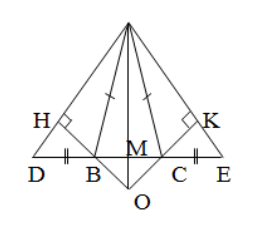
\includegraphics[width=0.4\textwidth]{17-5-lg.png}$$
    \begin{enumerate}
        \item $\triangle \mathrm{ABC}$ cân có $\mathrm{AB}=\mathrm{AC}$ nên: $\mathrm{ABC}=\mathrm{ACB}$\\[5px]
        Suy ra: $\mathrm{AB} D=\mathrm{ACE}$\\[5px]
        Xét $\in A B D$ và $\triangle A C E$ có:\\[5px]
        $\mathrm{AB} =\mathrm{AC}(\mathrm{gt}) \\[5px]
        \mathrm{ABD} =\mathrm{ACE}(\mathrm{CM} \text { trên }) \\[5px]
        \mathrm{DB} =\mathrm{CE}(\mathrm{gt}) \\[5px]
        \text {Do đó } \in \mathrm{ABD}=\Delta \mathrm{ACE}(\mathrm{c}-\mathrm{g}-\mathrm{c})\\[5px]
        \Rightarrow \mathrm{AD}=\mathrm{AE} \text { (2 cạnh tương ứng). Vậy } \Delta \mathrm{ADE} \text { cân tại } \mathrm{A} \text {. }$
        \item Xét $\triangle A M D$ và $\triangle A M E$ có:\\[5px]
        $\mathrm{MD}=\mathrm{ME}(\text{Do } \mathrm{DB}=\mathrm{CE}$ và $\mathrm{MB}=\mathrm{MC}$ theo $\mathrm{gt})$
        AM: Cạnh chung\\[5px]
        $\mathrm{AD}=\mathrm{AE} \text { (CM trên) }$\\[5px]
        Do đó $\triangle A M D=\triangle A M E(\mathrm{c}-\mathrm{c}-\mathrm{c})$\\[5px]
        $\Rightarrow M A D=M A E \text {. }$\\[5px]
        Vậy $A M$ là tia phân giác của $D A E$\\[5px]
        \item Vì $\triangle ADE$ cân tại A (CM câu a) nên $A D E=A E D$ \\[5px] 
        Xét $\triangle B H D$ và $\triangle C K E$ có:\\[5px]
        $B D H=C E K \text { (Do }  A D E=A E D \\[5px]
        \mathrm{DB}=\mathrm{CE} \text { (gt) } \\[5px]
        \Rightarrow \triangle B H D=\triangle C K E \text { (Cạnh huyền- góc nhọn) }$
        $
        \text { Do đó: } \mathrm{BH}=\mathrm{CK} \text {. }
        $
        \item Gọi giao điểm của $\mathrm{BH}$ và $\mathrm{CK}$ là $\mathrm{O}$.\\[5px]
        Xét $\triangle A H O$ và $\triangle A K O$ có:\\[5px]
        OA: Cạnh chung\\[5px]
        $\mathrm{AH}=\mathrm{AK}(\mathrm{Do} \mathrm{AD}=\mathrm{AE} ; \mathrm{DH}=\mathrm{KE} \text { (vì } \triangle B H D=\Delta C K E)) \\[5px]
        \Rightarrow \triangle A H O=\triangle A K O \text { (Cạnh huyền- Cạnh góc vuông) }$\\[5px]
        Do đó $O A H=O A K$ nên $\mathrm{AO}$ là tia phân giác của $K A H$ hay $\mathrm{AO}$ là tia phân giác của $D A E$.\\[5px]
        Mặt khác theo câu b) AM là tia phân giác của $D A E$.
        Do đó $\mathrm{AO} \equiv \mathrm{AM}$, suy ra 3 đường thẳng $\mathrm{AM}$; $\mathrm{BH}$; $\mathrm{CK}$ cắt nhau tại $\mathrm{O}$.
    \end{enumerate}
}
\end{bt}

